\documentclass[12pt,twoside, a4paper, twocolumn]{article}
\usepackage[utf8]{inputenc}
\usepackage[brazil]{babel}
\usepackage[margin = 0.5in]{geometry}
\usepackage{amsmath}
\usepackage{amsthm}
\usepackage{amssymb}
\usepackage{amsthm}
\usepackage{setspace}
\usepackage[americanvoltages,fulldiodes,siunitx]{circuitikz}
\usepackage{lipsum}
\usepackage{pgfplots}
\usepackage{ifthen}
\usepackage{adjustbox}
\usepackage[section]{placeins}
\usepackage{hyperref}
\usepackage{graphicx}
\usepackage{amsmath}
\usepackage{amsthm}
\usepackage{amssymb}
\usepackage{amsthm}
\usepackage{setspace}
\usepackage[americanvoltages,fulldiodes,siunitx]{circuitikz}
\usepackage{lipsum}
\usepackage{pgfplots}
\usepackage{ifthen}
\usepackage{adjustbox}
\usepackage[section]{placeins}
\usepackage{hyperref}
\usepackage{graphicx}
\usepackage{adjustbox}
 
\pgfplotsset{compat=newest}
\graphicspath{ {./images/} }
%  #1 color - optional #2 x_0 #3 y_0 #4 x_f #5 y_f #6 name - optional  #7 true if adding lines to axis
\newcommand{\drawvector} [9] [color=cyan] {
  \draw[line width=1.5pt,#1,-stealth](axis cs: #2, #3)--(axis cs: #4, #5) node[anchor=south west]{$#6$};
 \ifthenelse{\equal{#7}{true}}{
  \draw[line width=1pt,#1, dashed](axis cs: #4, #5)--(axis cs: #4, 0) node[anchor= north west]{$#8$};
  \draw[line width=1pt,#1, dashed](axis cs: #4, #5)--(axis cs: 0, #5) node[anchor=south east]{$#9$};
  }
  {}
}
\newcommand\deriv[2]{\frac{\mathrm d #1}{\mathrm d #2}}
\title{Quinto Relatório de Lab de Circuitos}
\author{Henrique da Silva \\ hpsilva@proton.me}
\date{\today}
\pgfplotsset{width = 10cm, compat = 1.9}
\begin{document}
\maketitle
\pagenumbering{gobble}
\newpage
%pagenumbering{roman}
\tableofcontents
\newpage



\section{Introdução}

\subparagraph*{Neste relatório vamos discutir um circuito com um AmpOp e dois capacitores que se comportara como um circuito RLC.}

\subparagraph*{Todos arquivos utilizados para criar este relatório, é o relatorio em si estão em:  \url{https://github.com/Shapis/ufpe_ee/tree/main/4th semester/lab circuitos}}


\section{Analise do circuito}

\subparagraph*{Podemos fazer a seguinte análise no nosso circuito:}

\begin{equation*}
    \begin{aligned}
         & \frac{V_a - V_i}{R_1} + \frac{V_a-V_0}{R_2} + \frac{V_a}{R_3}  + C1 \deriv{V_a}{t} = 0                                  \\
         & \frac{-V_a}{R_3} - C_2 \frac{V_0}{t} = 0                                                                                \\
         & V_a = -R_3 C_2 \deriv{V_0}{t}                                                                                           \\
         & V_a \left(\frac{1}{R_1} + \frac{1}{R_2} + \frac{1}{R_3}\right) + C_1 \deriv{V_a}{t} - \frac{V_0}{R_2} = \frac{V_i}{R_1} \\
         & R_3 C_2 \deriv{V_0}{t} K_1 + C_1 C_2 R_3 \deriv{\deriv{V_0}{t}}{t} + \frac{V_0}{R_2} = \frac{-V_i}{R_i}                 \\
    \end{aligned}
\end{equation*}

\subparagraph*{Que segue:}


\begin{equation*}
    \begin{aligned}
         & V_0(0) = - V_{C20}                                                             \\
         & \deriv{V_0}{t} = - \frac{V_{C10}}{R_3 C_2}                                     \\
         & V_a(t) = V_{C_1}(t) \rightarrow V_a(0) = V_{C10} = - R_3 C_2 \deriv{V_0}{t}(0) \\
         & V_{C_2}(t) = - V_0(t) \rightarrow V_0(0) = -V_{C20}                            \\
    \end{aligned}
\end{equation*}

\newpage

\section{Medições no laboratório}

\subsection{Valores reais das partes.}
\subparagraph*{Abaixo estao os valores medidos das partes utilizadas no experimento:}

\begin{center}
    \begin{tabular}{ |ccc| }
        \hline
        $R_1$ & $\rightarrow$ & $46.34K\varOmega$ \\
        $R_2$ & $\rightarrow$ & $32.21K\varOmega$ \\
        $R_3$ & $\rightarrow$ & $67.1K\varOmega$  \\
        $C_1$ & $\rightarrow$ & $1.05nF$          \\
        $C_2$ & $\rightarrow$ & $101.56nF$        \\

        \hline
    \end{tabular}
\end{center}

\subsection{Imagem da onda}

\begin{adjustbox}{scale=0.4}
    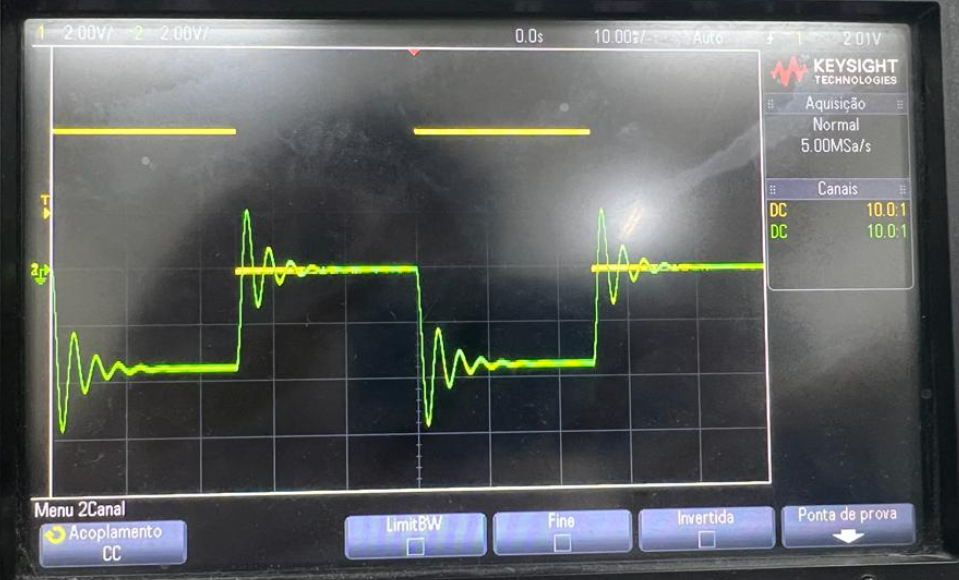
\includegraphics{Figure_1.png}
\end{adjustbox}

\subsection{Medicoes para o regime permanente}

\subparagraph*{Inicialmente medimos as tensoes nos capacitores para tempos longos, ou seja. Quando estao em regime permanente, e obtivemos o seguinte:}

\begin{equation*}
    \begin{aligned}
        V_{C10} = -3.5V \\
        V_{C20} = 0V    \\
    \end{aligned}
\end{equation*}

\subsection{Resposta natural}

\subparagraph*{Obtivemos que em resposta natural, o capacitor $C_1$ em $t_0$ tem uma tensao de $-3.5V$, ele oscila de maneira subamortecida ate tender a $0V$ em $t = \infty$.}

\subparagraph*{Ja o mesmo capacitor $C_1$ em resposta forcada, inicia em $0V$ e oscila de maneira subamortecida ate tender a $-3.5V$ em $t = \infty$.}

\subsection{Tempo de subida e descida}

\paragraph*{Utilizarei a frequencia $f = \frac{1}{8} \alpha = 41.4$ para todos experimentos a seguir. Isto nos dara tempo suficiente para a tensao estabilizar.}

\begin{center}
    \begin{tabular}{ |ccc| }
        \hline
        $\%V$      & $t_{subida}$ & $t_{descida}$ \\
        $t_{10\%}$ & $200\mu s$   & $720 \mu s$   \\
        $t_{90\%}$ & $200\mu s$   & $900 \mu s$   \\
        \hline
    \end{tabular}
\end{center}

\subsection{Overshoot}

\begin{center}
    \begin{tabular}{ |ccc| }
        \hline
        $\,$             & $Tempo$  & $Tensao$   \\
        $T_{overshootN}$ & $1.45ms$ & $2.15V$    \\
        $T_{overshootF}$ & $1.4ms$  & $-2.0625V$ \\
        \hline
    \end{tabular}
\end{center}

\newpage
\section{Atividades pós laboratoriais}

\end{document}